\documentclass[letterpaper,9pt]{report}
\usepackage{thesis}
\usepackage{url}
\usepackage{listings}

\usepackage[T1]{fontenc}
\usepackage[scaled]{DejaVuSansMono}

% For programming language keywords
\newcommand{\kw}[1]{{\lstinline[language=JavaScript]!#1!}}
\newcommand{\jsfile}[1]{{
    \begin{flushleft}
    \scalebox{1}{\lstinputlisting[language=JavaScript]{#1}}
    \end{flushleft}
}}


\lstdefinelanguage{JavaScript}{
  morekeywords=[0]{typeof, new, this, delete, throw, try, catch, function, return, switch,
            var, if, in, while, do, for, else, case, break, continue, with, finally},
  morekeywords=[1]{\_\_get\_\_, \_\_set\_\_, \_\_new\_\_, \_\_clone\_\_, \_\_delete\_\_, 
                   \_\_itr\_\_, \_\_str\_\_, \_\_type\_\_,\_\_\$call\_\_,\_\_\$apply\_\_,
                   \$arguments, \$arguments\_slice},
  ndkeywords={true, false, null, undefined},
  comment=[l]{//},
  morecomment=[s]{/*}{*/},
  basicstyle=\small\ttfamily,
  %stringstyle=\small,
  keywordstyle=[0]\bfseries,
  keywordstyle=[1]\itshape,
  morestring=[b]",
  showstringspaces=false
}

%\lstdefinelanguage{plain}{
%  keywords={},
%  ndkeywords={},
%  comment=[l]{//},
%  morecomment=[s]{/*}{*/},
%  morestring=[b]',
%  morestring=[b]"
%}



\begin{document}

\pagenumbering{roman}

% Fill in the title, author, degree name, department, and month/year.
% Upon completion, this should look like the following:
%\thesistitle
%	{Complicated and Important-Sounding Thesis Title}
%	{John P. Doe}
%	{Master of Science}
%	{Department of Computer Science}
%	{May 2009}
% The \thesistitle definition is in thesis.sty.  Other customizations
% can be made there.
\thesistitle
	{Harnessing Performance for Flexibility in a Virtual Machine for JavaScript}
	{Erick Lavoie}
	{Maîtrise en Sciences}
	{D\'epartement d'Informatique et de Recherche Op\'erationelle}
	{Décembre 2012}

%
\addcontentsline{toc}{chapter}{R\'esum\'e}
\begin{center}
\textbf{\large R\'esum\'e}
\end{center}


\vspace{1cm}
Les d\'eveloppements r\'ecents sur les machines virtuelles (MVs), en particulier
pour le language JavaScript, ont mis l'emphase sur la performance au d\'etriment
de la flexibilit\'e. Cela limite notre compr\'ehension du comportement dynamique
des programmes en rendant laborieuse l'instrumentation de MVs existantes. Les
approches pass\'ees consistaient \`a instrumenter manuellement un interpr\'eteur
commercial, limitant l'acquisition de donn\'ees longitudinale, \`a cause du co\^ut
\'elev\'e de maintenance de l'interpr\'eteur.
			
Ce m\'emoire montre que la flexibilit\'e peut \^etre r\'ecup\'er\'ee dans l'instrumentation
dynamique du mod\`ele objet et des appels de fonctions, \`a un niveau de
performance comp\'etitif avec un interpr\'eteur commercial r\'ecent, sans
modification de son code source. Notre approche consiste \`a ex\'ecuter une MV
m\'eta-circulaire, ciblant le langage source, sur une MV rapide. Pour \'evaluer
l'approche, nous proposons une MV pour JavaScript, nous pr\'esentons des exemples
d'instrumentation et nous comparons la performance, avec et sans
instrumentation, \`a l'interpr\'eteur SpiderMonkey et la MV bas\'ee sur un JIT de V8.
			
Nous croyons que la combinaison de simplicit\'e, de flexibilit\'e et d'efficacit\'e
de notre MV est unique. Elle est rendue possible par trois contributions:

\begin{itemize}
    \item L'unification des op\'erations r\'eifi\'ees du mod\`ele objet et des appels
        de fonctions autour d'une primitive unique de passage de message,
        compatible avec la derni\`ere version de JavaScript
    \item Une impl\'ementation efficace de la primitive de passage de message
        inspir\'ee par la m\'emoisation \textit{in situ}.
    \item Une repr\'esentation objet qui exploite les optimisations de
        m\'emoisation \textit{in situ} de la VM sous-jacente et le dynamisme du mod\'ele
        objet pour obtenir des op\'erations virtualis\'ees efficaces 
\end{itemize}

Mots-cl\'es: M\'eta-circularit\'e, Instrumentation, Dynamisme, Mod\`ele Objet,
Flexibilit\'e, Performance, Machine Virtuelle, JavaScript  

\addcontentsline{toc}{chapter}{Abstract}
\begin{center}
\textbf{\large Abstract}
\end{center}


\vspace{1cm}


%\include{text/abstract_non_technical}
%\addcontentsline{toc}{chapter}{Acronyms}
\begin{center}
\textbf{\large Acronyms}
\end{center}


\vspace{1cm}

\addcontentsline{toc}{chapter}{Remerciements}
\begin{center}
\textbf{\large Remerciements}
\end{center}

Un grand merci \`a mes colocataires des trois derni\`eres ann\'ees, J\'er\^ome,
Claire, Estelle puis plus tard No\"el ainsi qu'\`a mes ami(e)s en particulier
Awa et Bianka, qui ont \'et\'e aux premi\`eres loges pour partager mes joies et
frustrations mais surtout pour avoir offert un environnement qui m'a permis de
d\'ecrocher quand j'en avais besoin.

Merci \`a Paul (Khuong) et Paul (Raymond-Robichaud) pour les discussions
stimulantes, \'Etienne et David pour le partage de leur exp\'erience du milieu
acad\'emique, ce qui a bris\'e mon sentiment d'isolement aux moments o\`u j'avais
l'impression d'\^etre seul face \`a certaines difficult\'es.

Merci \'egalement \`a tous ceux qui sont pass\'es par le lab pendant mon s\'ejour, en
particulier Beno\^it, pour la co-cr\'eation de la version la plus \'epique d'un
Pacman 3D moustachu \`a laquelle j'aie particip\'e, Eric, Vincent et Benjamin pour
avoir d\'emontr\'e un int\'er\^et pour mes nombreuses "d\'emos" de versions interm\'ediaires
du syst\`eme ainsi que Maxime pour m'avoir montr\'e un calibre de programmation que
je n'avais pas connu jusqu'\`a mon entr\'ee au lab.

Merci au personnel administratif du d\'epartement d'informatique
et de recherche op\'erationnelle, en particulier Mariette Paradis, pour les
nombreux accomodements et les judicieux conseils prodigu\'es pour la navigation
au travers des requis administratifs inh\'erents \`a la poursuite d'\'etudes gradu\'ees
dans un contexte institutionnel. Cela a grandement simplifi\'e ma vie.

Merci \`a Bruno Dufour, qui aurait m\'erit\'e d'\^etre officiellement
co-directeur vu son niveau d'implication dans mon projet de ma\^itrise.
L'identification du probl\`eme d'instrumentation dynamique efficace est une
cons\'equence directe de nos discussions. L'instrumentation dynamique a fourni
un usage pratique \`a une solution qui \'etait en recherche d'un probl\`eme. Tu
es \'egalement le premier \`a avoir pleinement reconnu l'int\'er\^et
acad\'emique de mon travail.

Merci \`a Marc Feeley, mon directeur, d'avoir servi d'exemple sp\'ecifiquement
par son soucis du d\'etail et du mot juste ainsi que ses capacit\'es techniques
remarquables.  Bien que \,ca n'ait pas toujours \'et\'e intentionnel, merci
\'egalement de m'avoir sorti de ma zone de confort. Mes limites personnelles
ont \'et\'e dans certains cas repouss\'ees et dans d'autres cas raffermies. 

\tableofcontents

\addcontentsline{toc}{chapter}{List of Tables}
\listoftables

\addcontentsline{toc}{chapter}{List of Figures}
\listoffigures


\pagenumbering{arabic}
\chapter{Introduction}

\funnyquote{Impermanent are all component things,\\
They arise and cease, that is their nature:\\
They come into being and pass away,\\
Release from them is bliss supreme.}
{Mahaa-Parinibbaana Sutta \cite{1988last}}

Computer systems are constantly modified to satisfy the evolving needs of their
users. \textit{Flexible} systems can evolve faster than rigid systems by
placing fewer constraints on possible modifications, thus reducing the delay
between the birth of an idea and its actual realization in a working system.
Aiming for flexibility in the design of computer systems can make other
properties, such as performance, security and reliability, easier to obtain by
facilitating experimentation.

A \textit{virtual machine} (VM) is a program that simulates the behavior of a
computing machine.  The simulated machine might exhibit properties that do not
have physical equivalents. For example, by using a garbage collection
component, it can provide the illusion of infinite allocatable memory. Programs
executing on VMs inherit their properties and constraints, therefore making
them prime research objects to provide properties to an important number of
programs.

Recent research and development on VMs, especially for the JavaScript
language~\cite{js_spec}, has focused on performance, to the expense of
flexibility. Notably, it has hindered our understanding of the run-time
behavior of real-world programs by making instrumentation of existing VMs
laborious. The last published attempt at gathering empirical data for
JavaScript was a one-time effort, where researchers manually instrumented a
production interpreter to obtain execution traces~\cite{behavior_js}. However
this approach prevents the acquisition of longitudinal data because the burden
of maintaining the instrumented interpreter up-to-date is too demanding for any
research team to shoulder.

Fortunately, the very same gains in performance can be used to regain
flexibility, even on a rigid production VM. This dissertation shows that a
sophisticated run-time optimizer can be harnessed to provide flexible run-time
instrumentation of the object model and function-calling protocol at a
performance competitive with a state-of-the-art interpreter, without having to
modify the VM source code. Our approach consists in running a metacircular VM
targeting the source language, based on a message-sending object model, on top
of another fast VM. To demonstrate the approach, we provide a reference VM for
an existing programming language, JavaScript, we show the possibility of
instrumenting the object model operations and function calls and we finally
compare the performance with and without instrumentation to the SpiderMonkey
interpreter and V8 JIT-compiler based VM. 

Although there are existing systems for JavaScript targeting JavaScript as
their runtime, such as Google Caja to enforce security
invariants~\cite{Caja:2012}, Google Traceur to support the next version of
JavaScript on existing VMs~\cite{Traceur:2012} and JSBench to record execution
traces for automatic benchmark generation~\cite{Richards:2011}, we believe our
system is unique in its combinaison of design choices that makes it simple,
flexible and sufficiently efficient for data gathering of dynamic behavior. As
such, this dissertation contains three original contributions: 
\begin{itemize}
    \item The unification of the reified object model operations and
        function-calling protocol around a single message-sending primitive
        while preserving compatibility with the current version of JavaScript
    \item An efficient implementation of the message-sending primitive inspired
          by inline cache optimizations
    \item An object representation exploiting the underlying VM inline caches
          and dynamic object model to provide efficient virtualized operations
\end{itemize}

In addition to supporting the thesis above, we hope (1) to encourage future
language designs to provide features facilitating an efficient layered approach
to obtain flexibility and (2) the object representation will be used by other
language implementations seeking efficiency while targeting existing JS VMs.

\section{Flexibility}

Defining and evaluating flexibility is no easy task. The usage of the term
above appeal to the intuitive notion of a system easy to tailor to one's
particular usage by modifying, removing or replacing its components. Easy might
mean that there is few lines of code to modify to use a preconfigured option,
that there is few manipulations to perform in a user interface or that unplanned
extensions could be developed in a limited time.

While intuitive, this definition is not sufficiently objective to compare
different systems. It is tied to a subjective interpretation of efforts required to
perform modifications. For the remainder of this dissertation, I'll use a more
restricted definition of flexibility. A system will be considered flexible if
it exhibits the four following properties:

\begin{itemize}
    \item \textit{Open}. Its components' behavior can be modified by
        first-class data structures and the range of possible behavior is
        maximal. 

    \item \textit{Extensible}. Its components can be independently modified or
        replaced and they support incremental definitions. 

    \item \textit{Dynamic}. It can be modified at run time.

    \item \textit{Performant}. It is fast enough to provide instant feedback on
        user modifications.
\end{itemize}

There is a continuum of support for these four properties. For example, some
parts of a system might be open but not others.  I will not try to estimate the
relative contribution of each of these properties to the overall flexibility of
a system. I will instead evaluate systems on use cases for each of these
property individually. A system could be said to be more open than another one
but not more flexible unless it is clearly equally or more open, extensible,
dynamic and performant than another one.

\section{Virtual machine}

% definition
A \textit{virtual machine} is a program that simulates the behavior of a
machine, that may or may not have a physical implementation. It may be
identical to the physical machine on which it is executing, as is the case with
current commercial solutions used to execute different operating systems as user
processes, or it might be completely different, as is the case when executing a
high-level language such as JavaScript. In this latter case, the simulated
machine might exhibit properties that do not have physical equivalents.
For example, the illusion of infinite allocatable memory can be provided by
implementing a garbage collector algorithm.~\footnote{Note, that the available
working memory is still finite and limited by the underlying physical memory
available.} 

% relationship to an operating system
In theory, there is no significant difference between a VM and
an operating system.~\footnote{"An operating system is a collection of
things that don't fit into a language. There shouldn't be one." -- Dan
Ingalls~\cite{Ingalls1981}} They both act as a middle layer between the
underlying machine and programs. They both provide abstractions and
services common to all programs. In fact, VMs for high-level
languages have been made to execute directly on hardware. In practice, the
management of hardware peripherals, memory, processing units and network
interfaces has been associated with operating systems and the support for
higher-level features of programming languages has been associated with
dedicated VMs. This historical distinction has allowed a plethora
of languages to be available for application programmers by allowing language
implementers to focus on supporting the semantic of programming languages
instead of managing the physical machine resources.

% efficiency gap
The major drawback of simulating a computer is the important efficiency
difference between a physical and a virtual implementation, the latter possibly
being orders of magnitude slower then the former. Research on VM
implementation has contributed techniques to minimize this efficiency gap.
Various high-level languages, such as Java, JavaScript, Smalltalk, Scheme or
Prolog, can now execute efficiently on general purpose processors making VMs
practical for application development.

% scope
In this dissertation, I will focus on VMs constructed to support programming
languages on top of existing operating systems or VMs. I will ignore the
virtualization of operating systems or the management of physical resources.

VMs can be described by three languages:
\begin{itemize}
    \item \textit{Source language}. Language used by programs executing on the VM.
    \item \textit{Implementation language}. Language that describe the behavior of the VM.
    \item \textit{Target language}. Language of the machine on which the VM is executing.
\end{itemize}
These languages can be different. For example, current commercial VMs for
JavaScript (source language) are written in C++ (implementation language) and
execute on Intel X86 processors (target language). Special cases, which exhibit
noteworthy properties, exist when some or all of these languages are the same. 

When its source language and its implementation language are the same, a VM is
said to be \textit{metacircular}. Advantages of metacircularity are resource
sharing and uniformity of the runtime. For example, a memory manager used to
manage the internal data structures of a VM can be shared with the source
language runtime. Uniformity allows optimizations written for the source
language to also apply to the implementation language. In the context of an
open system, source language code can replace implementation language code to
modify the behavior of the VM. In the litterature, \textit{self-hosting} is
also used to describe metacircular systems. I'll restrict this latter term for
describing a system that is \textit{actually} used to produce new versions of
itself.  Therefore, a metacircular VM needing special extensions or
performance that it cannot provide still depends on an external machine to
produce a different version of itself and is not self-hosting. Self-hosting is
therefore more strict.  Self-hosting enables a faster evolution of the system
by allowing functionalities developed for the source language to apply to the
implementation language. It frees a system from the limitations of other
available systems that would be needed otherwise.

When its source language and its target language are the same, we usually
describe a VM as performing \textit{source-to-source} translation. This is
especially useful to provide additional or different properties to the
executing program while avoiding the implementation of complicated
functionalities, such as floating-point or regular expression support.  It can
be used to reduce a complicated language to a kernel language using only a
subset of all the functionalities offered in the source language. This is
especially useful when implementing mainstream languages possessing redundant
features acquired through backward-compatibility-constrained evolution. It may
ease reasoning about the program, facilitate instrumentation or exploit
optimizations written for some functionalities to accelerate others.

When its implementation language and its target language are the same, an
\textit{executable} VM can execute on a machine without requiring any external
support. Few VMs are implemented directly in a target low-level language unless
an executable VM is needed but no translator from a high-level language to the
target low-level language are available. When translators are available,
executable VMs are usually the result of an automatic translation from a high-level
description.

When all languages are the same, I will say a VM is \textit{platonic}.  I would
argue that a platonic VM is possibly the simplest that could be built for a
given language. Only the elements of interest in the language can be acted
upon, the others can be left as is without having to provide an implementation
in a lower-level language.  Tools supporting the source language can be used to
inspect, modify and debug the VM, creating a highly productive environment.
Optimizations for the new functionalities can target existing optimisations of
the source language to efficiently implement new functionalities and properties
without having to specify low-level mecanims that would otherwise be required.
It greatly simplifies exploration of novel ideas. More importantly, it suggests
a metric to evaluate the cost of providing fonctionalities or properties that
are not available in the original source language: the overhead of executing an
original source program on the VM compared to bare execution on the reference
machine. When the overhead is small, it is an indication that the functionality
\textit{can} be implemented efficiently using known techniques. However, if the
overhead is high, the functionality \textit{may} be implemented using known
techniques or techniques yet to be invented.

In this dissertation, using a platonic JS VM, I show that the object model
presented is practical performance-wise by showing that is has a low
overhead on given benchmarks for every object operation it implements. 

\section{JavaScript}

JS is a dynamic language, imperative but with a strong functional component,
and a prototype-based object system similar to that of Self.

A JS object contains a set of properties (a.k.a. fields in other OO languages),
and a link to a parent object, known as the object's prototype. Properties are
accessed with the notation \kw{obj.prop}, or equivalently \kw{obj["prop"]}.
This allows objects to be treated as dictionaries whose keys are strings, or as
one dimensional arrays (a numeric index is automatically converted to a
string).  When fetching a property that is not contained in the object, the
property is searched in the object's prototype recursively. When storing a
property that is not found in the object, the property is added to the object,
even if it exists in the object's prototype chain. Properties can also be
removed from an object using the \kw{delete} operator. JS treats global
variables, including the top-level functions, as properties of the global
object, which is a normal JS object.

Anonymous functions and nested functions are supported by JS. Function objects
are closures which capture the variables of the enclosing functions. Common
higher-order functions are predefined. For example, the \kw{map}, \kw{forEach}
and \kw{filter} functions allow processing the elements of an array of data
using closures, similarly to other functional languages. All functions accept
any number of actual parameters. The actual parameters are passed in an array,
which is accessible as the \kw{arguments} local variable. The formal parameters
in the function declaration are nothing more than aliases to the corresponding
elements at the beginning of the array. Formal parameters with no corresponding
element in the array are bound to a specific undefined value.

JS also has reflective capabilities (enumerating the properties of an object,
testing the existence of a property, etc.) and dynamic code execution
(\kw{eval} of a string of JS code).  The next version of the standard is
expected to add proper tail calls, rest parameters, block-scoped variables,
modules, and many other features.

Initially, our research initiative chose JS as a research object because it is
widely used to write web applications and there is a performance gap between
benchmarks executing on the fastest implementations and compiled with C/C++
compilers, suggesting there are techniques to be found to close the gap.
During exploration of VM implementation techniques, the dynamic nature of the
language was found to be particularly well-suited to base a flexible design
around it and initiated the work presented here.

\section{Object Model}

An object model is a set of object kinds, their supported operations and the
time at which those operations can be performed.  Examples of object kinds are
arrays, numbers, associative arrays and classes.  Examples of operations are
object creation, addition, removal or update of properties as well as
modification of the inherintance chain. Examples of time for performing
operations are \textit{run time}, when a program is executing, \textit{compile
time}, when a program is being compiled or \textit{edit time}, when a program's
source code is being modified. An object model structures programs to obtain
properties on the resulting system such as security, extensibility or
performance. Most object models for programming languages provide an
inheritance mecanism to facilitate \textit{extensibility} by allowing an object
to be defined incrementally defined in terms of an existing object.

Different languages have different object models. \textit{Class-based}
object-oriented languages use \textit{class} objects to describe the properties
and the inheritance chain of \textit{instance} objects. For example, C++ class
objects exist only at compile time. Property values can be updated at run time.
Properties can only be added or removed at edit time and all their accesses are
verified at compile time. Java use run-time objects to represent classes and
allow new classes to be added at run time.  Classes cannot be modified at run
time unless their new definition is reloaded through the debugger API. Ruby
class objects exist at run time and new properties can be added also at run
time. \textit{Prototype-based} object-oriented languages forego the difference
between class and instance objects. Objects and their inheritance chain is
defined directly on objects. Self and JavaScript object properties can be
added or removed at run time. 

\textit{Message sending} is an operation that invoke a behavior on an object by
executing a program associated to a given message.  A message can exist at run
time and be an object like any other or it can exist only at compile time.
Message sending \textit{decouples} the intention of a program from its
implementation by adding a level of indirection between the invocation and the
execution of a given behavior. This indirection allows the behavior to change
during a program's execution. Therefore, it is a source of \textit{dynamism}.

Some languages call the program associated to a message, a \textit{method
implementation}, the message, a \textit{method name} and the act of sending a
message, \textit{method calling}. This terminology is closely tied to an
implementation strategy where the implementation is a function, the method name
is a compile-time symbol and the method call is a lookup followed by a
synchronous function call in the same address space. I will prefer the
message-sending terminology because it is more abstract and would easily
accomodate an asynchronous calling mecanism that could happen between different
address spaces (i.e. machines). 

A message-sending object model is an object model that takes message sending as
its primitive operation. It defines every other operation in terms of message
sends. By doing so, every other operation of the object model becomes dynamic,
i.e. it can change at run time.

An object model defined in terms of itself is an object model where every
component required to implement the object model operations are themselves
objects. For example, the behavior of objects might be functions, the messages
might be symbols and classes might associate symbols to functions. By
recursively defining the object model in terms of itself, it becomes
\textit{open} to modification from regular object operations.

A message-sending object model defined in terms of itself combines both the
dynamism of message sending with the openness of recursivity. By providing
every operation through a message send and having every component part of the
object model, it effectively encapsulate its implementation strategy,
facilitating its evolution. By being based on a message sending primitive, the
optimization effort can be focused on this primitive and run-time information
can be used to specialize the behavior invoked, providing an opportunity for
\textit{performance}. 

The next pages show how a message-sending object model for JS defined in terms of
itself provides \textit{openness}, \textit{dynamism}, \textit{extensibility}
and \textit{performance} and empirically evaluate its practicality for building
\textit{flexible} virtual machines.

\section{Meta-Circularity}
\subsection{VM Paradigm vs Instrumentation}
Closed world assumption vs Open world assumption

\section{Features required from the host runtime}


\section{Outline}
\begin{itemize}
    \item The next chapter presents previous work on flexible computer systems.
    \item Chapter~\ref{chap:Design} explains the design of the object model
    independently of the implementation or the target language of the VM.
    \item Chapter~\ref{chap:Implementation} explains implementation
    peculiarities for a particular target and implementation language, JS.
    \item Chapter~\ref{chap:Optimizations} describes the optimization
    techniques used to remove much of the dynamic overhead of the design,
    tailored to a particular JS implementation.  
    \item Chapter~\ref{chap:Flexibility} presents use cases in modifying the VM
    that are either difficult or impossible to do with existing JS
    implementations.
    \item Chapter~\ref{chap:Complexity} evaluates the complexity of the
    resulting system using the number of source lines of code as a proxy.
    \item Chapter~\ref{chap:Performance} compares my implementation with a
    state-of-the-art implementation to establish the overhead of providing the
    flexibility.  
    \item The conclusion presents the lessons I learned in building, whole or
    part, three VMs during the course of this research project. I conclude with
    recommandations on browser behavior that would allow this design to
    serve as a basis for web pages to provide their own runtime, relaxing
    current hard-constraints on web application evolution.
\end{itemize}

\chapter{Previous Work}
\label{chap:PreviousWork} 

\funnyquote{Those who cannot remember the past are condemned to repeat it.} 
{George Santayana, $1863-1952$}

The work described in this dissertation started as an exploration of the
possibilities offered by an object model based on the open, extensible object
model by Piumarta and Warth~\cite{Piumarta:2008}. In this chapter, we first
trace back the original sources of core ideas that eventually influenced our
implementation by organizing them around four themes, \textit{openness},
\textit{extensibility}, \textit{dynamism} and \textit{performance} and by
focusing on issues pertaining to the object model and function-calling
protocol. We finally review other existing systems that perform dynamic
instrumentation of JavaScript and compare them to Photon.

\section{Historical roots}

The previous work is presented in chronological order to provide a sense of
evolution and temporal distance. Throughout the exposition, we make explicit
the elements that inspired our work and we contrast the elements that are
different.

\subsection{Openness}

The meaning of open depends on what is being qualified. Perhaps the most common
usage is open \textit{source}. It refers to accessibility of the text
representation, or source code, that was used to produce the system.
Accessibility of the source code and development tools allows a motivated
person to modify the text representation and generate a new version of the
system incorporating the change. However, it says nothing about the nature and
the number of changes that are be required to obtain a desired behavior.

We use the term open as an implementation qualifier. It therefore means that
the behavior of the system can be modified by first-class data structures, e.g.
closures. The range of behavior modifications allowed by an implementation
characterizes the degree of openness.

The earliest account of the need for open implementations seems to be made by
Shaw and Wulf in 1980~\cite{Shaw:1980}. In it, they argue that the approach
taken to define abstract data types should also be used to define the behavior
of language operations, namely to separate the \textit{specification} from its
\textit{implementation}. They identify storage layout, variable handling,
operator semantics, dynamic storage allocation, data structure traversal and
scheduling and synchronization as areas ripe to benefit from being opened.
Compared to our focus on opening the object model operations and
function-calling protocol, these elements are closer to the machine execution
model than to the language's semantics. 

Smith worked concurrently on similar areas with a different approach. He first
asked how a system could reason about its own inference processes. This was an
inherently philosophical question. In his PhD dissertation in
1982~\cite{Smith:1982}, he answered it, not only by clarifying the notions
behind reflectivity, but also by showing how an interpreter for Lisp could be
built to satisfy those notions. His work planted the seeds for an influential
line of research. Compared to Shaw and Wulf work, it directly addressed the
semantic implications of opening implementations while they merely suggested
that some elements should not be bound early without giving any indication on
how to define the semantics of a programming language to do so.  The notion of
reflection is also stronger because it implies the ability to modify the
implementation from within the language itself. Among the notions Smith
introduced, we use the \textit{causal connection} criteria to think about
JavaScript semantics in section~\ref{sec:AugmentedFunctionCalling}. This
criteria says that a data structure is causally connected to the behavior of a
system if changing the data structure changes the behavior of the system.

In a landmark OOPSLA paper in 1987~\cite{Maes:1987}, Maes showed how to bring
reflection to object-oriented programming languages through meta-objects.
These objects were shown to encapsulate various elements of the language
implementation. Later in 1991, Ramano Rao introduced the open implementation
term to replace the reflection architecture term that was previously in use to
emphasize that not only language implementations can be open but also
applications~\cite{Rao:1991}. Then, a methodology for designing open
implementations was suggested by Maeda and al.~\cite{Maeda:1997}, first by
taking an existing closed implementation and then by progressively opening all
the elements of interest. This line of work took the conceptual underpinnings
of reflection and integrated it with other language developments at the time,
showing that it could be used in practice to build not only programming
languages but whole systems around those principles. In the same spirit, our
work applies the open implementation idea to a mainstream language, JavaScript,
and solves the associated design and performance issues associated with it.

\subsection{Extensibility}

The term extensible means that a VM's components can be independently modified or
replaced, that new components can be supported without having to modify
existing components and they can be incrementally defined in terms of existing
components. Encapsulation and modularity covers a subset of that definition. 

A major breakthrough in structuring the definition of computer systems was the
introduction of the notion of \textit{inheritance} in 1966 by Dahl, Myrhaug and
Nygaard in the Simula 67 language~\cite{Dahl:1968}. The language had the notion
of classes and objects and new classes could be defined in terms of existing
classes through its inheritance mechanism. The language had a major influence on
the design of Smalltalk~\cite{Kay:1993} and C++~\cite{Stroustrup:2007}.

Another major idea for extensibility was the notion of \textit{encapsulation},
initially called \textit{information hiding} by Parnas in
1972~\cite{Parnas:1972}. In his paper, he argued that instead of decomposing
systems by subroutines performed, they should be decomposed such that modules
encapsulate key design decisions, in a way that is as independent as possible
from other decisions.  Later Dijkstra argued for a similar idea which he named
\textit{separation of concerns} and applied it not only to system design but
also problem-solving and general thinking. The first occurrence of the term
seems to be found in 'A Discipline of Programming'~\cite{dijkstra:1976}. The
object-oriented community finally adopted encapsulation to describe the idea,
when applied to computer systems.

In the object-oriented community, a class-based approach to object
decomposition was favored until Lieberman proposed in
1986~\cite{Lieberman:1986} to use a prototype-based approach to implement
shared-behavior. This latter mechanism was shown to be more expressive since it
could be used to implement an equivalent class-based mechanism but the opposite
was not possible. This had a major influence on the design of
Self~\cite{Ungar:1987} which later influenced the design of JavaScript.

The object representation presented in section~\ref{sec:ObjectRepresentation}
exploits prototype-based inheritance and a method-based behavior definition
that allows encapsulation of design decisions made for optimizations. It allows
instrumentations to be written for our system with minimal knowledge about its
inner working. Our work does not contribute new ideas for extensibility but
uses powerful existing ones to simplify its implementation and evolution.

\subsection{Dynamism}

Dynamism has seen an increasing usage through the popularization of dynamic
languages. Again, the actual meaning of dynamism in dynamic languages is
fuzzy. The common thread however is the presence of \textit{late-binding} of
some aspects of the programming language, namely deferring until run time the
actual computation required to implement a given functionality.

There is an overlap between the work presented in the previous section and this
one because ideas for extensibility evolved in parallel with ideas for
dynamism.

The earliest account of dynamic strong typing seems to be in the initial Lisp
paper by McCarthy in 1960~\cite{McCarthy:1960}. In it, the type of variables
was enforced (strong typing) at run time (dynamic typing). Later, polymorphism
through message-sending, or the ability of a given identifier to invoke
different behavior during execution, was pioneered both in its asynchronous
version in the Actor model by Hewitt in 1973~\cite{Hewitt:1973} and in its
synchronous version by the Smalltalk crew, led by Kay between 1972 and
1976~\cite{Kay:1993}. The main difference between the asynchronous version and
the synchronous version is that in the former, the flow of control returns to
the sender before the message has been processed while it waits for the message
to be processed in the latter. In both cases, message-sending is the primitive
operation on which all the other operations are based.

Going back to Smith in 1982~\cite{Smith:1982}, in his work on reflection, we
can also note that the emphasis was put on the ability to reflect upon the
dynamic behavior of programs, which would later be called behavioral reflection
although the term Smith used was procedural reflection.

Finally, one important characteristic of prototype-based inheritance, as
explained by Lieberman in 1986~\cite{Lieberman:1986} is its dynamic nature. The
prototype of an object is known and can change during program execution.

JavaScript uses dynamic strong typing and prototype-based inheritance.  We
exploit these characteristics for dynamic instrumentation. In our work, the
idea of using message-sending as a foundation was inspired by Smalltalk  and
the dynamic nature of the instrumentation we perform owes a great deal to the
behavioral reflection work. We use reflection capabilities in
chapter~\ref{chap:Flexibility} to show how to change the semantics of object
model operations.

\subsection{Performance}

Dynamic languages have had the reputation of being slow and inefficient. This
is changing as mainstream languages incorporate more dynamic features and
considerable engineering efforts are targeted at improving their performance.
Apart from optimizations deriving from idioms of a particular language, two
historical papers provide the ground works we used.

In 1984, Deutsch an Schiffman introduce the inline cache technique to optimize
method dispatch on class-based object-oriented languages~\cite{Deutsch:1984}.
The technique uses dynamic code patching to memoize the class of the receiver
to store the lookup result at the call site for faster later execution. In
1989, Chambers and al. generalized the technique to prototype-based languages
by introducing the concept of \textit{map}, an implicit class constructed by
the implementation as objects are created and modified during
execution~\cite{self}.

Both of these techniques were inspirations for the optimizations we explain in
section~\ref{sec:EfficientImplementation}.

\section{Instrumenting JavaScript VMs}
%The last years have seen increasing interest from the research community toward
%JavaScript and web applications. Most relevant to our work here are empirical
%evaluations of JavaScript dynamic behavior. Ratanaworabhan and
%al.~\cite{jsmeter} as well as Richards and al.~\cite{behavior_js} have
%respectively shown that benchmarks do not correspond to the behavior of real
%Web applications and that JavaScript applications are more dynamic than what
%was previously thought. Both papers are sources of experiments to perform on
%JavaScript VMs and serve as a starting point in thinking about the capabilities
%required for a VM aiming for instrumentation. We replicate a part of the object
%model instrumentation from the second paper in our performance evaluation in
%Chapter~\ref{chap:Performance}.

%Richards and al. have also proposed another system, JSBench to record execution
%traces of JavaScript execution on websites, that can be replayed as standalone
%benchmarks~\cite{Richards:2011}. Their system performs a source-to-source
%translation of JavaScript source code and proxies some operations of the
%language to record traces. Although they claimed the overhead introduced by
%their system for the benchmarks presented was less than 10\% and depended on
%the number of proxy objects created, no comprehensive evaluation of the
%performance of their instrumentation strategy was done. It is therefore
%impossible to compare the performance overhead of our approach with theirs from
%the evaluation results they published. Further investigation would be required
%to see if our approach could be practical to record execution traces in the
%same manner.

%\section{Virtual Machines running on top of JavaScript Virtual Machines}
%Various virtual machines have been built
%\begin{itemize}
%    \item Google Traceur compiler
%    \item Mozilla Shumway
%    \item Google Caja
%\end{itemize}

Kikuchi et al. reported on the real-world applicability of instrumenting
JS to enforce security policies~\cite{Kikuchi:2008}. They discuss
instrumentation of web applications  by intercepting and rewriting incoming
JS code in web pages by a proxy server operating in-between a client
browser and a web server. Their work is complementary to ours.
Their rewriting strategy could be adjusted to use Photon's execution model and
applied to other problems than security policy application.  Their rewriting
strategy also targeted object model operations and function calls and they
reported an impact of less than a factor of two in execution time on web
applications, such as GMail. However, these results were obtained in 2008, at
the beginning of JIT compilation strategy adoption in web browsers. Given our
performance evaluation, a higher ratio would be expected on modern VMs. 

Sandboxing frameworks for JS, such as Google Caja~\cite{Caja:2012},
BrowserShield~\cite{Reis:2007} and ADSafe~\cite{ADSafe:2013} guarantee that
guest JS code cannot modify the host JS environment outside of
a permitted policy. We focus here on Google Caja as a representative candidate.
The Caja sandbox provides a different global object to the guest code and
performs a source-to-source translation to ensure that all operations on host
objects are mediated by proxies enforcing a user-defined security policy.
Photon also provides a different global object to the running application and
performs a source-to-source translation to mediate object operations through
proxies. However, it is done to simplify reasoning about instrumentations while
providing an acceptable level of performance. Our sandboxing strategy does not
need to be as stringent, therefore we deem acceptable the possibility of
leaking the native objects by accessing the \kw{__proto__} property.
Documentation of the run-time performance penalty of their approach is sparse.
However, the authors do report a \~{ }\factor{17} slowdown on EarleyBoyer when
running over Rhino
1.6.7\footnote{https://code.google.com/p/google-caja/wiki/Performance}, a
somewhat slower JS VM than the Firefox interpreter (in comparison, Photon has a
\factor{9.53} slowdown for EarleyBoyer on the Firefox interpreter).

JSBench~\cite{Richards:2011} performs instrumentation of object operations and
function calls for recording execution traces of web applications that can be
replayed as stand-alone benchmarks. Instrumented operations then call global
functions, in a way similar to the esprof prototype we built
(Section~\ref{sec:esprof}). Its authors report an impact on performance that is
``barely noticeable on most sites'' even when running in interpreter mode on
Safari. JSBench instrumentation is specially tailored to the task of recording
benchmarks while Photon aims to be a general instrumentation framework.

 The idea of using aspect-oriented programming for profiling tasks has
been successfully used in the past, although some limitations of the model
have been identified (e.g., \cite{BinderEtAl:CPE11}).
AspectScript~\cite{Toledo:2010} has similar aims as Photon, namely providing
for JS a general interface for dynamic instrumentation of object operations
and function calls.  It uses a source-to-source translation scheme with a
single \textit{reifier} primitive which is analogous to our
\textit{message-sending} primitive. They document a scoping strategy that
allows targeting a single object or function, instead of all objects
globally, which is more flexible than Photon's current strategy. We believe
that Photon could be extended similarly.  Compared to our instrumentation
interface, they use the dynamic weaving of aspect formalism instead of our
``operations as methods'' approach. Because of the use of the aspects
formalism, their approach provides better encapsulation of the instrumentation
strategy at the expense of flexibility and performance. We executed the latest
version of AspectScript against the V8 benchmarks, and found it to be between
\factor{10} and \factor{454} slower than Photon on Safari. Additionally, only
four of the benchmarks ran without errors.

Js.js~\cite{Terrace:2012} is a JS port of the Firefox interpreter
compiled using the Emscriptem C++ to JS compiler.  It is intended for sandboxing web applications. The
resulting JS interpreter then runs in the browser on top of an existing VM.
However, this is a heavy-weight approach with a significant performance overhead.
The authors report slowdowns between \factor{100} and \factor{200} for most cases with worst cases of
\factor{600} on SunSpider benchmarks. The large slowdown can be attributed to the
full simulation of a native interpreter in JS. Photon avoids
reimplementing features of the language outside object operations and function
calls. The resulting implementation is both faster and simpler to instrument.

Other approaches target the host VM for efficiency reasons.
JSProbes~\cite{jsprobes:2012} is a series of patches to the Firefox interpreter
that allow instrumentations to be written in JS and target pre-defined probe
points, such as object creation, function calls and implementation events such
as garbage collector start and stop events. JSProbes provides much of the same
properties as Photon at a much lower execution overhead and with additional
information about implementation events that are inaccessible to Photon. It is
however less flexible since for the same language operations, JSProbes is
limited to a fixed set of predefined events while Photon allows the semantics
of operations to be changed. Unfortunately, targeting a VM implementation
requires maintenance to follow the upstream modifications. At the time of
writing, maintenance of JSProbes has stopped, making the approach unavailable
in practice.  In a different setting, Lerner et al. explored the requirement
for implementing aspect support in an experimental
JIT-compiler~\cite{Lerner:2010}. They reported a simpler and more efficient
implementation than other aspect-oriented approaches. Their work was intended
to inform possible ways to open native implementations to instrumentation with
an aspect formalism. So far, no production VM implements aspects, which makes
this approach unavailable in practice. Photon does not require modifications to
the host VM. It therefore does not add to the maintenance cost of production
VMs to be usable in practice. 

Recently a new low-level implementation of the JavaScriptCore
interpreter optimized for performance became available.  In our tests
on the V8 benchmark suite, the new interpreter is roughly \factor{3}
faster than the Firefox interpreter.  The performance gains are
attributable to using an assembly language.  As this new interpreter
matures its complexity will likely increase, negating most of the
simplicity usually attributed to interpreters.  This makes the task of
instrumenting the new JavaScriptCore interpreter much harder to
achieve and maintain, and consequently, the Firefox interpreter is
currently the only JS interpreter that is reasonably fast and
sufficiently easy to instrument.  

The Narcissus JS in JS interpreter implementation by Mozilla reifies all the
language operations of the language. It could be instrumented by inserting
hooks in the corresponding case statements of the main interpretation loop.
However, compared to Photon, Narcissus is much slower. Unfortunately, none of
the V8 benchmarks could be executed. However, on a micro-benchmark stressing
the function calling protocol, it was two orders of magnitude slower than
Photon. The overhead can be attributed to the reification of activation records
for function calls. In contrast, Photon uses the execution environment of the
host VM to provide better performance.

\chapter{Design}
\label{chap:Design}

\section{Goals}

\section{Inspiration}

\section{Contributions}

\subsection{JavaScript Extensions}

\subsection{Dynamic Evolution support}

\subsection{Reflexion support}


\chapter{Flexibility}
\label{chap:Flexibility}

\funnyquote{You must be shapeless, formless, like water. When you pour water in a
cup, it becomes the cup. When you pour water in a bottle, it becomes the
bottle. When you pour water in a teapot, it becomes the teapot. Water can drip
and it can crash. Become like water my friend.}
{Bruce Lee}

Any system exhibits particular compromises between opposing goals. Some
constraints derive from the nature of the problem a particular system is trying
to solve. Different problems might have conflicting constraints. Therefore, a
given system cannot be the ultimate answer to life, the universe and everything
to everybody. It follows that to assert the flexibility of a system, we need to
choose particular use cases and leave out others. This chapter presents the
uses cases we chose to support and how they can be implemented using our
design.

%TODO: Explain that for most examples, we will directly use the implementation
%      language, while it could also have been possible to expose some primitive
%      operations to the source language

We will see different examples modifying the base system to adapt it to
particular use cases. The examples are written either in the implementation
language of the VM, which has a direct access to the object representation and
the execution environment or in the source language, which does not and
correspond to the execution environment of user-supplied code. In other words,
the implementation language is executed directly on the host VM and the source
language is first translated to execute in a virtualized environment like
regular source code. A comment line at the beginning of each example explicitly
states if the example is written in the implementation language or the source
language.

We first explore how to obtain object model operation information by redefining
their corresponding methods.  We then see how to obtain a dynamic call graph by
redefining the \kw{call} method on functions. Both of these support our thesis,
by showing how the object model and the function calling protocol can be
instrumented. Finally, we discuss ways to enforce runtime invariants used to
catch common programming mistakes to show that although our focus was on
building instrumentation infrastructure, the resulting system has broader
applicability than the context in which it was developed.

\section{Obtaining object model operation information}
\label{sec:ObjectModelInstrumentation}

Given a good approximation of the performance cost of JS operations, such as
property accesses and object creation, we might be interested in estimating the
performance of an application by computing the number of run-time occurrence of
each of these operations.

The design of the system makes it easy to do by wrapping the method
implementing the semantic operation with a function incrementing a counter.  In
the following example, we do it for property accesses, property assignations
and property deletions. The following example shows an example of
instrumentation code for the object model, expressed in the
implementation language:

\jsfile{listings/object-model-instrumentation.js}

This instrumentation can be exercised with the following example, written in
the source language:

\jsfile{listings/object-model-instrumentation-test.js}

It should give a count of one for property assignations, a count of two for
property accesses and a count of three for property deletions.

Notice that the instrumentation is granular in time, namely it can be activated
and interrupted at any moment.  To cover the entire application execution,
instrumentation need simply be activated before an application is actually
started. 

\section{Obtaining a dynamic call graph}

A dynamic call graph is a data structure encoding the calling relationship
between functions, occurring during the execution of a program. For example, if
a function \kw{a} calls a function \kw{b}, the \textit{a calls b} relationship
will be registered in some way. 

Dynamic call graphs can be used to determine the code coverage of unit tests as
well as to provide detailed runtime information for code comprehension,
run-time optimizations and analyses of source code. 

Context-insensitive call graphs do not encode the calling context of a call,
while context-sensitive call graphs do. For context-insensitive call graphs, we
might represent functions as nodes and calling relationships as edges.
Context-sensitive call graphs could represent functions as multiple nodes,
depending on their respective callers. For the sake of simplicity, we will
consider a context-insensitive call graph for the remainder of this example. 

As seen previously in the design chapter~(\ref{chap:Design}), function calls
origin from four sources in the language: global function calls, method calls,
indirect calls through \kw{call} and \kw{apply} and direct calls to functions
stored in variables.~\footnote{As discussed in the conclusion, they also occur
implicitly in the standard library. These are not supported for now.} By
redefining the \kw{call} and \kw{apply} methods, we can intercept every call
made from these four origins.

The following program will be traced and exhibits every case enumerated
above. Four different functions are declared and two are initially called:

\jsfile{listings/callgraphexample.js}

By inspection, we can see that \kw{a} calls \kw{b}, that \kw{b} calls no other
function, that \kw{c} recursively calls itself but no other function and \kw{d}
is not called nor calls another function. We would expect a call graph like the
one shown in Figure~\ref{fig:CallGraph} to model those relationships.

\begin{figure}[htb]
\begin{center}
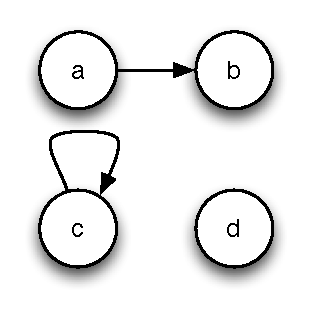
\includegraphics{figures/callgraph}
\caption{\label{fig:CallGraph} Call Graph for example code}
\end{center}
\end{figure}

A context-insensitive analysis requires a single node by function. Therefore,
we can store the profiling information directly on the functions themselves.
This way it avoids the complexity associated with maintaining separate data
structures and maintaining a correspondence between functions and those data
structures.

\subsection{Protecting the profiling code in a critical section} 

A \textit{critical section} usually refers to a section of code in a
multi-threaded program in which the system guarantees that no preemption will
occur. By analogy, we use the term to refer to a section of code in a profiled
program in which the system guarantees that no profiling occurs.

By using a critical section, we solve the issue of having the profiling code
being profiled. It is important to avoid profiling the profiling code, not only
because it pollutes results but mostly because it can introduce
\textit{meta-stability} issues, namely that performing an operation in the
profiling code might call back into the same operation being profiled, creating
an infinite loop.

A critical section can be implemented by introducing a flag that controls
whether profiling occurs or not. Just before the profiling code starts
executing, the flag is set and right after the profiling code ends the flag is
reset. It can be done with a boolean variable if the section needs not be
reentrant or with a integer otherwise.

When profiling JS function calls, we need to be cautious about the different
ways the flow of control can be manipulated by the callee. In JS, a function
can return either normally through its explicit or implicit return statement or
by raising an exception. Fortunately, JS provides a \kw{finally} construct that
guarantees that however the flow of control leaves a try block, the \kw{finally}
block will always be executed. We can therefore perform pre-call operations in
a \kw{try} block and perform post-call operations in a corresponding
\kw{finally} block.

The next requirement is to be able to intercept every function call in the
program. Our design makes it easy by reducing every occurrence of function calls
to sending the message \kw{call} or \kw{apply} to the called function, whether
it is global, local or is a method. We can further implement \kw{call} in terms
of \kw{apply}, which gives us a single point of instrumentation for the whole
system. By redefining the \kw{call} and \kw{apply} method on the root function,
we can profile the whole system.

The only problem left by this approach comes from the circularity introduced by
having every JS object operation and function invocation performing a
\kw{call}. It means that no primitive operation in the source language can be
used to perform a call. We solve it by performing the instrumentation in the
implementation language.~\footnote{Extensions to the source language could also
have been made, in which case the source language could have been used to the
same effect.}

The next example introduces two instrumentation primitives as global functions
in the source language, \kw{startCallInstrumentation} and
\kw{stopCallInstrumentation}. When called, the instrumentation function
initializer redefines the \kw{call} and \kw{apply} methods on the root function
and uses the \kw{before} and \kw{after} source-language functions to perform
pre- and post-call operations.  By virtue of the critical section, any operation
performed by \kw{before} and \kw{after} will not be profiled:

\jsfile{listings/dyn-call-graph-instr.js}

This definition has an interesting property: the initialization of the call
instrumentation is atomic and will take effect the next time a call is
performed but will not affect any function currently in the calling context.
Likewise, the instrumentation can be changed or stopped on-the-fly but the
previous instrumentation will still performs its post-call operations on
functions currently in the calling context.

The previous listing was essentially an extension of the implementation to
allow function call instrumentation. The next listing uses that extension to
build a dynamic call graph. It registers all called functions on a shadow stack
as well as the calling relationship between the function on top of the shadow
stack and the called function. A predicate is used to avoid registering calls
to functions that do not have an identifier (\kw{\_\_id\_\_}
property).~\footnote{Identifying functions in JavaScript is non-trivial because
some of them are anonymous, they might be stored in more than one variable and
their variable name might conflicts with other locally-defined variable names
elsewhere in the program. For this particular example, an extension to the
source language was made that uses the global variable name as an identifier. A
different naming strategy might be used without impact on the code presented.}
The \kw{dynCallGraphResults} function prints the call graph in the dot language for
visualization. This instrumentation can be expressed in the source language:

\jsfile{listings/dyn-call-graph-mon.js}

The instrumentation performed will output the expected call graph as shown in
previous section. Running both the extension and the instrumentation on the
example code given at the beginning of the section will output the correct
dynamic call graph.

\section{Enforcing run-time invariants}

Instead of extending the behavior of operations to perform instrumentation, the
next examples \textit{modify} the semantics of the original operation to provide
a different behavior, with the goal of enforcing run-time invariants. This goes
beyond our thesis to provide a glimpse of the usefulness of the system beyond
instrumentation tasks.

\subsection{Ensure that all accesses are made to existing properties}

The default semantics of property access in JS specifies that accessing
a non-existing property should return \kw{undefined}. It has the unfortunate
consequence that the presence or absence of a property on an object is
ambiguous: if an existing property has \kw{undefined} as a value, we cannot
tell if the property is present or not by the return value of the property
access operation. Combined with the automatic conversion of values for most
operations, an unintended missing property on an object might cause obscure
bugs to crop up later in the program.

We can provide a \textit{fail early} semantics to the property access operation
by raising an exception if a property is not present. This can be done easily
by replacing the \kw{\_\_get\_\_} operation on the root object. The following
example uses the implementation language to have access to the object
representation methods directly:

\jsfile{listings/failearlyget.js}

The next example performs the same operation but shows that this modification 
can be expressed in the source language instead:

\jsfile{listings/failearlyget-source.js}

In both examples, having separate cases for the presence of a property with an
\kw{undefined} value and an absent property, an exception can be thrown only in
the second case. A similar method could be used to check arrays for
out-of-bounds accesses or deletions that could migrate the representation from
dense to sparse.

\subsection{Ensure that a constructor always returns the object it received}

The semantics of object construction in JS can be surprising. When creating an
object with a call to a function with the \kw{new} operator, a new empty object
is created behind the scene and the function will be called with a \kw{this}
value bound to the created object. When the function returns, the return value type 
is inspected. If it is an object, the \kw{new} expression will yield the
returned object. However, if it is a primitive value, the \kw{new} expression
will yield the object created before the call to the function.

This behavior guarantees that an object will always be returned and allows
constructors to be written more succinctly by omitting the \kw{return}
statement. However, it might also be a source of run-time errors if a
constructor is later modified and an object is unintentionally returned.

We can dynamically change the semantics of the construction operation to throw
an error if an object different than the original object created is returned by
the constructor, in the source language:

\jsfile{listings/constructorcheck.js}

The two examples show the power of opening an implementation, beyond mere
instrumentation. The fact they could both be written in the source language
with a minimal amount of knowledge of the implementation brings the
possibilities of modifying the language semantics to non-implementers.

Now that we have seen what we gained from a flexible implementation, we will
see how much performance that cost us.

\chapter{Optimizations}
\label{chap:Optimizations}

\emph{``We should forget about small efficiencies, say about 97\% of the time: premature optimization is the root of all evil. Yet we should not pass up our opportunities in that critical 3\%. A good programmer will not be lulled into complacency by such reasoning, he will be wise to look carefully at the critical code; but only after that code has been identified''}

-- Donald Knuth \\

\section{Inline primitive operations}

\section{Inline caching of message sends}

Invariants: 
\begin{itemize}
    \item Parent objects never share a map (a map change happens when a child is created)
    \item values are only cached when found on a parent object
    \item value caches are only present on parent objects
\end{itemize}

Problems:
\begin{itemize}
    \item Caching a "call" message
\end{itemize}

\section{Semantic optimization}

\chapter{Performance}
\emph{``There is a deep difference between what we do and what mathematicians
do. The "abstractions" we manipulate are not, in point of fact, abstract. They
are backed by real pieces of code, running on real machines, consuming real
energy and taking up real space. To attempt to completely ignore the underlying
implementation is like trying to completely ignore the laws of physics; it may
be tempting but it won't get us very far.''}

-- Gregor Kiczales~\cite{Kiczales92towardsa} \\

\label{chap:Performance}

The last section introduced techniques to reduce the run-time overhead of the
object model. We now evaluate the actual run-time and memory-usage overhead
incured by the additional flexibility. We will see that it compares favorably
to the performance of a state-of-the-art interpreter, making the approach
viable for instrumentation. Additionnally, the actual figures obtained will
allow the reader to evaluate if this approach could be applied to other usage
scenarios.

The next section explains the methodology used to evaluate the performance of
the system. We then present the baseline performance (without instrumentation)
obtained on different systems for common benchmarks. We then see the
performance impact of a chosen instrumentation and we conclude with an
interpretation of the results. 


\section{Methodology}

We compare three different systems:
\begin{itemize}
    \item Photon running over V8 (V8's full optimizations)
    \item V8 (full optimizations)
    \item SpiderMonkey interpreter (JIT disabled)
\end{itemize}

V8 was chosen to host Photon because preliminary tests showed the system to be
faster on it. The additional speed is attributed to the ability of the runtime
to do function inlining, On-Stack-Replacement and the presence of fast Garbage
Collectors. Other VMs are catching up on features so we anticipate that in the
near future they could probably be used interchangeably. We compare Photon to
V8 to quantify the performance cost incured by our approach. This really gives
the cost of harnessing some performance to provide more flexibility to the
system.  We finally compare to a popular state-of-the-art interpreter to argue
that our approach can be used wherever a manual instrumentation of that
interpreter could have been performed. 

In choosing the systems to compare, we eliminated a few current alternatives.
We assume that when faced with the task of instrumenting production code to
obtain run-time data, manually instrumenting a JIT-compiler would be deemed too
complex to be cost-effective in terms of development time. At the time of
writing, a new interpreter became available, namely JavaScriptCore's
low-level interpreter.  However, we argue that the only real instrumentation
alternative right now would be SpiderMonkey's interpreter because the
JavaScriptCore low-level interpreter is implemented in an assembly dialect to
obtain performance gains. As this new interpreter matures, we speculate that
its complexity will increase, negating most of the simplicity usually
attributed to interpreters.~\footnote{Should the reader still consider the
alternative of instrumenting JavaScriptCore's low-level interpreter instead,
she should know that in our tests, on V8's benchmarks, JavaScriptCore low-level
interpreter was roughly three times faster than SpiderMonkey's interpreter.}
Finally, we do not show performance results for Narcissus, Mozilla's JavaScript
in JavaScript interpreter, because the latest version would not run either
SunSpider or V8 benchmarks.

To assess performance, we use the SunSpider and V8 benchmark suites, since they
became the \textit{de facto} standard to compare JS VM performance. They both
come with their own different evaluation methodology. We used the methodology
of each benchmark suite without modification to make our results comparable to
other results obtained elsewhere for other systems. All the benchmarks were run
unmodified. However, the date benchmarks from SunSpider were omitted because
they relied on using \kw{eval} to access local variables, which is not
supported by our current compiler.  Since Photon's local environment use the
underlying VM's local environment (it is not reified), we believe that
supporting this feature in the future will not affect significatively the
performance results presented here.

We focus on two metrics, total running time and the maximum heap size to
respectively measure run-time performance and memory usage. Running time is
measured either directly, in the case of SunSpider's benchmarks or indirectly
through a score, in the case of V8's benchmarks. Memory usage is only used to
estimate the overhead of Photon compared to V8.

We present results in two different groups, the baseline performance and the
instrumented performance.  The baseline performance is used to measure the
minimal overhead of the approach.  This is important to assess the viability of
the approach because a baseline overhead that would be too high could make the
approach unusable in the majority of cases, independently of the other
characteristics of the system. The instrumented performance is used to measure
the impact of instrumentation on the baseline performance. It is common
knowledge that instrumenting an interpreter has little impact over its overall
performance (this was verified by Richards and al. when they instrumented
JavaScriptCore~\cite{behavior_js}). However, our approach might be more
sensible to instrumentation. We therefore show the impact of a basic
instrumentation on the performance of Photon. We used the V8 benchmarks because
they perform more and more varied operations in a single benchmark than the
SunSpider benchmarks. We count the number of occurrence at run time of each
reifed object-model operation. We chose this particular instrumentation because
it is simple, it covers every object model operation and it can be used to
reproduce the object read, write or delete proportion figure
from~\cite{behavior_js}.

% TODO: Provide machine specs and versions for both d8 and spidermonkey

% TODO ?? Provide graphic with confidence intervals and means
\section{Baseline Performance}

\subsection{Running Times}

\subsubsection{V8 benchmarks}

\input{/Users/erick/Recherche/photon-js/results/baseline/v8/time/table.tex}

\subsubsection{SunSpider benchmarks}

\input{/Users/erick/Recherche/photon-js/results/baseline/sunspider/time/table.tex}

\subsection{Memory Usage}

\subsubsection{V8 benchmarks}

\input{/Users/erick/Recherche/photon-js/results/baseline/v8/memory/table.tex}

\subsubsection{SunSpider benchmarks}

\input{/Users/erick/Recherche/photon-js/results/baseline/sunspider/memory/table.tex}

\section{Instrumented Performance}

\subsection{Running Times}

\subsubsection{V8 benchmarks}

\input{/Users/erick/Recherche/photon-js/results/instrumented/v8/time/table.tex}

\subsubsection{SunSpider benchmarks}

\input{/Users/erick/Recherche/photon-js/results/instrumented/sunspider/time/table.tex}

\subsection{Memory Usage}

\subsubsection{V8 benchmarks}

\input{/Users/erick/Recherche/photon-js/results/instrumented/v8/memory/table.tex}

\subsubsection{SunSpider benchmarks}

\input{/Users/erick/Recherche/photon-js/results/instrumented/sunspider/memory/table.tex}


\section{Interpretation}


\chapter{Conclusion}
\label{chap:Conclusion}

%\funnyquote{The end is the beginning of all things,\\
%Suppressed and hidden,\\
%Awaiting to be released through the rhythm\\
%Of pain and pleasure}
%{Jiddu Krishnamurti}

\funnyquote{Now this is not the end. It is not even the beginning of the end. But
it is, perhaps, the end of the beginning.}
{Winston Churchill}


The preceding chapters explained how a metacircular VM targeting its source
language, based on a message-sending object model could provide flexible
run-time instrumentation of the object model and function-calling protocol at a
baseline performance within a factor of two of a state-of-the-art interpreter,
by harnessing a sophisticated run-time optimizer, without having to modify the
underlying VM source code. The motivation for the work stems from the effort
involved with the current approach, namely to manually instrument a production
interpreter and maintain it up-to-date. This dissertation explained how to
solve the core technical issue behind this state of affairs. 

However, there is still some work to be performed to \textit{actually} use
those results to gather empirical data about JavaScript programs. At the same
time, the approach suggests other possible uses which might be worth exploring.
In the next sections, we discuss the limitations of the current prototype, with
regard to its JavaScript implementation, and we identify how the approach could
be broadly applied by improving upon our current results.

\section{Limitations}

The limitations of our current prototype come from JavaScript peculiarities
that might be eliminated if the next versions of the standard were
allowed to relax strict backward compatibility. Another option would be
to perform run-time checks to ensure they never arise.  However, we conjecture
that the resulting system is more useful by relaxing the strict adherence to
the behavior expected from current VMs for substantial performance gains.  In
the face of numerous quirks and warts in the design of the JavaScript language,
it is more important to provide a useful and powerful system, but potentially
incorrect, than an irremediably slow but correct one.

\subsection{Accessing the \kw{__proto__} property leaks the internal representation}

This limitation can affect the soundness of the program. This could have been
solved at the design stage of JavaScript, if the access to the prototype of an
object has been made through a method call, such as \kw{getPrototype()} instead
of by accessing the \kw{__proto__} property. This is a problem of mixing
meta-level with base-level information.

The problem can be mitigated with no run-time penalty by detecting, at
compile-time, accesses to the \kw{__proto__} property and calling the object
representation \kw{getProtype} method instead. However, the possibility of
dynamically generating the \kw{__proto__} name renders it unsound. It
is yet to be seen if this actually happens in the wild.

\subsection{Meta-methods can conflict with regular methods if they have the same name}

This limitation will be solved in the next version of the standard, when
unforgeable names will be available in user space.  Until then, we can rely on
seldom used names to minimize possible conflicts with existing code.

\subsection{Setting the \kw{__proto__} property throws an exception}

This might be fixed by invalidating all caches should the prototype of an
object change. A more sophisticated mechanism could be devised if the operation
is frequent.

\subsection{Operations on \kw{null} or \kw{undefined} might throw a different exception}

When trying to access a property or call a method on the \kw{null} or
\kw{undefined} value, VMs for JS throw an exception telling the user that the
property or the method does not exist on the object. Our current design reifies
property accesses as a call to the \kw{get} method on the object representation
and calls as a call to the \kw{call} method, \textit{once the object operation
has been cached}. If the receiver is \kw{null} or \kw{undefined} the exception
will tell of a missing method that is different from the property or the method
called.

This problem actually only happens when instrumenting incorrect programs. It
might not be a problem at all when browsing the web. Otherwise, it would be
possible to test for \kw{null} or \kw{undefined} on every operations, at a
substantial run-time cost.

Another option would be to change the exception being raised by adding test and
patch code for that particular exception at every catch site, at a
potentially more reasonable cost depending on the actual usage of the catch
construct.

This is fundamentally a problem of non-uniformity in the object model. It would
not exist if every value was an object.  This could be fixed in a subsequent
revision of JavaScript by providing auto-boxing of \kw{null} and
\kw{undefined}, in a similar fashion as what is done for other primitive types,
and adding a "does not understand" handler for property accesses and method
calls that could be overwritten. The default behavior could be to raise an
exception when accessing, setting or deleting a property or calling a method.
The prototype object for \kw{undefined} and \kw{null} could then have methods that
raise proper exceptions.

\subsection{Limited support for eval}

Our compiler does not support accessing the local environment of a function
from evaluated code. This can be fixed by maintaining on functions the
environment information. This environment can then be provided to our compiler,
when it is called during an \kw{eval} operation.

\subsection{Function calls implicitly made by the standard library are not intercepted}

Functions passed to the standard library are wrapped to remove the extra
arguments introduced by our compilation strategy. Should the need to intercept
those calls arise, the wrappers could perform a message send instead of a
direct call.
 
\section{Future work}

The obvious short term work would be to package the system in a browser
extension for Firefox or Chrome and use it to try to replicate the results
obtained on the dynamic behavior of JavaScript programs~\cite{behavior_js}, to
see if they still hold and try the instrumentation on more than just the 100
more popular websites. Then we could extend the instrumentation to cover not
only the object model operations and function calls but also the binary, unary,
control-flow and reflexive operations.

We believe there is much more potential to the current approach. The
biggest open question is how close we can come to native performance while
providing flexibility unavailable in the vanilla implementation. We compared
ourselves to a state-of-the-art interpreter because this is what is being used
for instrumentation nowadays. Similar performance is therefore enough for
obtaining information about the dynamic behavior of JavaScript programs. 

We argue that as virtual machines for dynamic languages become faster and
incorporate more sophisticated optimization techniques, the implementation
techniques for layered VMs should become worthy of research efforts since they
have the potential to provide an efficient way of supporting numerous languages
with limited efforts. This dissertation is a step in that direction.

Also, there could be qualitative improvements if the performance was much
better, by opening whole new possibilities of applications.  In the next
sections, we reflect about possible approaches to improve efficiency
using known techniques.

\subsection{Improve compilation speed}

Our OMeta-based compiler~\cite{Warth:2007} can be significantly slow during the
parsing stage. If compilation speed becomes critical, it could be replaced with
a different algorithm or the OMeta runtime and compiled code could be
optimized.

\subsection{Allow a finer-grained redefinition of meta-methods}

Object-model operations can only be redefined on the root object, mostly to
simplify the tracking mechanism. A more sophisticated tracking mechanism could
allow object model operations to be redefined for subsets of all objects by
redefining the operation at the appropriate place on the inheritance hierarchy.

\subsection{Efficient instrumentation}

There are two major areas for optimizations: the baseline performance of the
system and the performance while the code is instrumented. We briefly touch
upon each of them. 

\subsubsection{Improve the baseline performance}

The easiest known technique that would be worth trying to replicate in a
metacircular setting is the dynamic recompilation of the source code based on
type-feedback obtained during execution. It would further allow the
specialization of the code to the actual types occurring during execution and
the removal of message-sending caches for operations that have not been
redefined.

Our current object representation makes it easy by wrapping the function being
executed.  The function could be replaced at run time with a specialized
version. This could eliminate type tests and specialize functions used as
constructors. Our current inline cache design allows the accumulation of
arbitrary information which could be used for that purpose.

The other technique to be tried is the object representation method
specialization presented in the design section. Further gains could be had if
both the lookup and the argument specialization were combined in a single
method.

\subsubsection{Provide mechanisms to optimize the instrumentation code}

First, the system internals currently use a memoization protocol to specialize base
operations. By exposing the mechanism to user code, this would allow analyses to
specialize their behavior based on previous executions. This could notably be
used to avoid performing operations in expensive data structures the second
time.

Second, the system could offer a better granularity of instrumentation.
Currently, instrumenting a base operation applies to all objects. However, if
we could target only a subset of objects and handle that subset at the cache
level, we could avoid the instrumentation cost for a majority of objects. This
could be done by implementing the equivalent of polymorphic inline caches and
having a finer-grained tracking mechanism for cache states.


%\subsection{Real-time analysis of the behavior of JavaScript programs}
%
%A sufficient performance could allow a real-time analysis of the behavior of
%JavaScript programs. Compared to the log and analyze approach previously
%done~\cite{behavior_js}, this could provide a qualitatively different
%experience.
%
%This could be used by web developers to develop an intuition about the
%performance cost of various operations. This could also be used by the
%JavaScript committee to develop a better idea of what features are actually
%used across the web and could allow the deprecation of features that are never
%used.
%
%\subsection{Simplification of production VMs}
%
%Some little-used features (or quirks!) of the JavaScript languages hold back
%the performance that could be achievable and are maintained for
%backward-compatibility reasons. Those features could be provided by a
%metacircular VM through newer and better performing features.  The
%metacircular VM could be loaded lazily only when the old features are actually
%invoked.
%
%\subsection{Server-side instrumentation}
%
%A server could dynamically choose to send an instrumented version of its
%JavaScript code to gather information about the actual usage made by users of
%the application. While executing, the instrumented library could "phone home"
%to send back profiling information. However, due to access restrictions in the
%browser, a server configuration is required to permit the direct communication
%of the instrumented code with the library developer server.
%
%\subsection{Library-based profiling}
%
%It is currently hard for library developers to know precisely what
%functionalities are actually used and in which context. It could be possible to
%provide a pre-instrumented library version, tailored to the questions the
%library developers would like to be answered that other web developers could
%use in their web pages. 
%
%\subsection{Server code instrumentation}
%
%%The emergence of NodeJS as a server environment obviously allows the system to
%gather information about server-side code.
%
%\subsection{Security invariants monitoring}
%
%Instrumentation could be performed to enforce security invariants instead of
%only logging operations. 


\addcontentsline{toc}{chapter}{Bibliography}
\bibliography{ref}


% If you have no appendices, remove the following two lines.
% If you have more appdences, add them as necessary.
% \appendix
% \chapter{Appendix title}
\label{apdx:somelabel}
This is Appendix~\ref{apdx:somelabel}.

You can have additional appendices too
(\emph{e.g.}, \texttt{apdxb.tex}, \texttt{apdxc.tex}, \emph{etc.}).
If you don't need any appendices, delete the appendix
related lines from \texttt{thesis.tex} and the file names
from \texttt{Makefile}.


\end{document}
